% ============================================================
%  Sistem Akuisisi Fotogrametri Otomatis Berbasis UR5
%  Dokumentasi Teknis Proyek
%  Kompilasi: pdflatex (jalankan 2x untuk daftar isi)
% ============================================================
\documentclass[11pt,a4paper]{article}

% ---------- Page geometry & typography ----------
\usepackage[a4paper,margin=2.3cm,top=2.5cm,bottom=2.5cm]{geometry}
\usepackage[T1]{fontenc}
\usepackage[utf8]{inputenc}
\usepackage{charter}
\usepackage[scaled=0.92]{helvet}
\usepackage{microtype}
\usepackage{parskip}

% ---------- Graphics, color, layout ----------
\usepackage{graphicx}
\usepackage{xcolor}
\usepackage{tikz}
\usepackage{booktabs}
\usepackage{array}
\usepackage{tabularx}
\usepackage{enumitem}
\usepackage{caption}
\usepackage{float}
\usepackage{pdfpages}

% ---------- Headers, sections, links ----------
\usepackage{fancyhdr}
\usepackage{titlesec}
\usepackage[hidelinks]{hyperref}

% ---------- Code listings ----------
\usepackage{listings}

% ---------- Indonesian labels ----------
\renewcommand{\contentsname}{Daftar Isi}
\renewcommand{\figurename}{Gambar}
\renewcommand{\tablename}{Tabel}
\renewcommand{\appendixname}{Lampiran}
\renewcommand{\refname}{Referensi}

% ---------- Color palette ----------
\definecolor{accent}{HTML}{1F3A68}      % deep navy
\definecolor{accentLight}{HTML}{4A6FA5} % softer blue
\definecolor{rule}{HTML}{B7C2D6}        % light divider
\definecolor{mute}{HTML}{6B6B6B}        % muted gray
\definecolor{bgcode}{HTML}{F4F6FA}      % code background
\definecolor{kw}{HTML}{1F3A68}          % keyword
\definecolor{cmt}{HTML}{6B6B6B}         % comment
\definecolor{str}{HTML}{8A4A1F}         % string

% ---------- hyperref setup ----------
\hypersetup{
    colorlinks=true,
    linkcolor=accent,
    citecolor=accent,
    urlcolor=accentLight,
    pdftitle={Sistem Akuisisi Fotogrametri Otomatis Berbasis UR5},
    pdfauthor={Dokumentasi Proyek},
    pdfsubject={Robotika, Computer Vision, Fotogrametri},
    pdfkeywords={UR5, Fotogrametri, WebODM, OpenCV, Robotika}
}

% ---------- Section styling ----------
\titleformat{\section}
  {\Large\bfseries\color{accent}}
  {\thesection.}{0.6em}{}
  [\vspace{2pt}{\color{rule}\titlerule[0.8pt]}]
\titleformat{\subsection}
  {\large\bfseries\color{accent}}
  {\thesubsection}{0.6em}{}
\titleformat{\subsubsection}
  {\normalsize\bfseries\color{accentLight}}
  {\thesubsubsection}{0.6em}{}
\titlespacing*{\section}{0pt}{18pt}{6pt}
\titlespacing*{\subsection}{0pt}{12pt}{4pt}

% ---------- Caption styling ----------
\captionsetup{
    font={small},
    labelfont={bf,color=accent},
    labelsep=period,
    justification=raggedright,
    singlelinecheck=false
}

% ---------- Header / footer ----------
\pagestyle{fancy}
\fancyhf{}
\renewcommand{\headrulewidth}{0pt}
\renewcommand{\footrulewidth}{0pt}
\fancyfoot[L]{\footnotesize\color{mute}Sistem Akuisisi Fotogrametri UR5}
\fancyfoot[R]{\footnotesize\color{mute}\thepage}

% ---------- Listings style ----------
\lstdefinestyle{clean}{
    backgroundcolor=\color{bgcode},
    basicstyle=\ttfamily\footnotesize,
    keywordstyle=\color{kw}\bfseries,
    commentstyle=\color{cmt}\itshape,
    stringstyle=\color{str},
    breaklines=true,
    showstringspaces=false,
    frame=none,
    xleftmargin=10pt,
    framexleftmargin=10pt,
    aboveskip=10pt,
    belowskip=10pt
}
\lstset{style=clean}

% ---------- Convenience macros ----------
\newcommand{\code}[1]{\colorbox{bgcode}{\texttt{\small #1}}}
\newcommand{\fig}[3][0.92\linewidth]{%
  \begin{figure}[H]
    \centering
    \includegraphics[width=#1]{figures/#2}
    \caption{#3}
    \label{fig:#2}
  \end{figure}
}

% ============================================================
\begin{document}

% ---------- Title page ----------
\begin{titlepage}
    \thispagestyle{empty}
    \begin{tikzpicture}[remember picture, overlay]
        \fill[accent] (current page.north west) rectangle ([yshift=-10.2cm]current page.north east);
        \fill[accentLight] ([yshift=-10.2cm]current page.north west) rectangle ([yshift=-10.45cm]current page.north east);
        \fill[accentLight] ([xshift=-3.5cm,yshift=-0.9cm]current page.north east) rectangle ([xshift=-0.9cm,yshift=-1.05cm]current page.north east);
    \end{tikzpicture}

    \vspace*{2.5cm}
    \begin{flushleft}
        {\color{white!85!black}\fontsize{11}{13}\selectfont\textsc{Dokumentasi Teknis Proyek}}\\[14pt]
        {\color{white}\fontsize{30}{36}\selectfont\bfseries Sistem Akuisisi}\\[6pt]
        {\color{white}\fontsize{30}{36}\selectfont\bfseries Fotogrametri Otomatis}\\[6pt]
        {\color{white}\fontsize{30}{36}\selectfont\bfseries Berbasis UR5}\\[22pt]
        {\color{accentLight}\fontsize{13}{17}\selectfont\itshape
        Pipeline akuisisi citra ter-trigger robot untuk rekonstruksi 3D\\
        dengan OpenCV, relay I/O, backend Bun/Elysia, dan WebODM}
    \end{flushleft}

    \vspace{2.2cm}

    \begin{flushleft}
        {\color{accent}\textsc{\small Lingkup Proyek}}\\[6pt]
        {\color{rule}\hrule height 0.6pt}\vspace{6pt}
        \begin{tabularx}{\linewidth}{@{}p{2.4cm}X@{}}
            \textbf{Domain}     & Integrasi robotika, \textit{computer vision}, fotogrametri \\[2pt]
            \textbf{Robot}      & Universal Robots UR5 (lengan kolaboratif 6-DOF) \\[2pt]
            \textbf{Sensor}     & Webcam USB NEMESIS (terpasang pada \textit{end-effector}) \\[2pt]
            \textbf{Trigger}    & Digital output DO[0] $\rightarrow$ relay/input board, pin 33 \\[2pt]
            \textbf{Software}   & C++ / OpenCV, libcurl, Bun + Elysia, web UI, WebODM \\[2pt]
            \textbf{Output}     & Dataset 16 citra $\rightarrow$ rekonstruksi padat 273{.}505 titik \\[2pt]
            \textbf{Kualitas}   & 16/16 citra teregistrasi, rata-rata \textit{reprojection error} 0{,}84 piksel \\
        \end{tabularx}
    \end{flushleft}

    \vfill
    {\color{rule}\hrule height 0.4pt}
    \vspace{6pt}
    {\color{mute}\footnotesize Dokumentasi ini disusun sebagai bukti portofolio. Seluruh gambar, log terminal, dan laporan kualitas WebODM direproduksi dari deployment aslinya.}
\end{titlepage}

% ---------- Table of contents ----------
\thispagestyle{empty}
\makeatletter
\renewcommand\l@section[2]{%
  \ifnum \c@tocdepth >\z@
    \addpenalty\@secpenalty
    \addvspace{0.8em \@plus\p@}%
    \setlength\@tempdima{2.0em}%
    \begingroup
      \parindent \z@ \rightskip \@pnumwidth
      \parfillskip -\@pnumwidth
      \leavevmode \bfseries\color{accent}
      \advance\leftskip\@tempdima \hskip -\leftskip
      #1\nobreak\hfil \nobreak\hb@xt@\@pnumwidth{\hss #2}\par
    \endgroup
  \fi}
\makeatother
\tableofcontents
\newpage

% ============================================================
\section{Ikhtisar Proyek}

Proyek ini menghadirkan \textbf{sistem akuisisi fotogrametri ter-trigger robot} yang lengkap, di mana lengan Universal Robots UR5 secara otonom bergerak mengelilingi objek target melalui \textit{waypoint} yang telah diprogram dan memberi sinyal ke \textit{daemon} C++ kustom untuk mengambil citra di setiap titik henti. \textit{Dataset} hasil capture kemudian diserahkan ke \textbf{WebODM} untuk direkonstruksi menjadi model 3D padat. Hasilnya adalah \textit{workflow} tertutup yang membawa operator dari sekadar \emph{``tekan tombol start''} hingga \emph{model padat 273.505 titik} tanpa perlu menekan tombol shutter atau menyusun pose secara manual.

Proyek ini mengintegrasikan empat domain teknik yang biasanya terpisah --- robotika industri, digital I/O level rendah, \textit{computer vision}, dan perangkat berbasis web --- ke dalam satu \textit{pipeline} yang koheren. Antarmuka pengguna berbasis web menjadi \emph{front-face} sistem sehingga operator non-developer pun dapat melakukan preview kamera, memulai sesi capture, mengunggah dataset, dan menampilkan model 3D di browser.

\fig[0.55\linewidth]{ur5_camera_setup.jpeg}{Pengaturan perangkat keras lengan robot UR5 dengan webcam NEMESIS yang dipasang di dekat end-effector untuk akuisisi citra fotogrametri otomatis.}

% ============================================================
\section{Latar Belakang dan Rumusan Masalah}

\textit{Workflow} fotogrametri konvensional untuk pemindaian objek umumnya mengandalkan operator manusia yang berjalan mengelilingi target sambil membawa kamera, mengatur framing setiap pengambilan secara manual, dan memastikan adanya overlap yang cukup antar citra berurutan. Pendekatan ini memunculkan tiga masalah berulang di lingkungan laboratorium atau bengkel:

\begin{itemize}[leftmargin=1.4em,itemsep=2pt]
    \item \textbf{Baseline tidak konsisten.} Pengambilan dengan tangan menghasilkan variasi jarak, ketinggian, dan kemiringan yang berbeda-beda, sehingga \textit{reprojection error} membengkak saat \textit{bundle adjustment}.
    \item \textbf{Repeatability rendah.} Objek yang sama yang di-capture oleh dua operator berbeda menghasilkan rekonstruksi yang berbeda secara kasat mata, sehingga \textit{pipeline} sulit divalidasi.
    \item \textbf{Padat tenaga.} Mengambil 16--40 sudut pandang yang terdistribusi dengan baik memerlukan beberapa menit perhatian penuh per objek.
\end{itemize}

Lengan kolaboratif UR5, dipasangkan dengan kamera \textit{end-effector} yang tetap dan \textit{daemon} capture yang di-\textit{trigger} via digital I/O, menyelesaikan ketiga masalah tersebut sekaligus: pose menjadi deterministik, repeatable, dan operator manusia keluar dari \textit{loop} sejak program mulai berjalan.

% ============================================================
\section{Tujuan Sistem}

Sistem dirancang berdasarkan tujuan terukur berikut:

\begin{enumerate}[leftmargin=1.6em,itemsep=2pt]
    \item Mengambil citra secara \textbf{otomatis} di setiap waypoint UR5, hanya menggunakan digital output bawaan robot sebagai \textit{trigger} --- tanpa perlu lapisan ROS tambahan.
    \item Mendeteksi \textit{trigger} dengan cara \textbf{polling relay/input board via HTTP}, sehingga \textit{daemon} capture dapat berjalan di laptop Linux mana pun yang berada pada LAN yang sama.
    \item Menghasilkan \textbf{dataset citra bernomor} pada disk (\code{dataset/images/img\_000XX.jpg}) yang siap diunggah langsung ke WebODM.
    \item Menyediakan \textbf{web UI} yang menampilkan preview kamera \textit{live}, kontrol start capture, upload dataset, dan akses 3D viewer.
    \item Merekonstruksi objek hasil capture di WebODM dengan rata-rata \textit{reprojection error} di bawah satu piksel (\textbf{sub-pixel}).
\end{enumerate}

% ============================================================
\section{Arsitektur Sistem}

Sistem disusun mengikuti prinsip pemisahan tanggung jawab yang jelas: robot bertanggung jawab atas pergerakan, relay board atas sinyal \textit{trigger}, \textit{daemon} C++ atas kamera, dan \textit{backend} atas orkestrasi dengan WebODM. Gambar~\ref{fig:repository_structure.png} memperlihatkan bagaimana \textit{codebase} ditata mengikuti pemisahan tersebut.

\fig[0.78\linewidth]{repository_structure.png}{Struktur repositori yang disederhanakan, menunjukkan modul perangkat lunak utama: backend API, camera interface, dan user interface.}

\subsection{Lapisan arsitektur}

\begin{description}[leftmargin=1.4em,itemsep=2pt,style=nextline]
    \item[Lapisan motion (UR5)] Menjalankan urutan \textit{waypoint} yang telah diprogram mengelilingi objek dan men-toggle digital output DO[0] pada setiap pose.
    \item[Lapisan signal (Relay/Input board di \texttt{192.168.200.219})] Membaca jalur DO[0] pada pin input 33 dan mengekspos statusnya via HTTP pada \code{/input}.
    \item[Lapisan capture (\texttt{camera\_interface}, C++)] \textit{Daemon} berbasis OpenCV yang berjalan \textit{headless}; bertugas mem-polling \textit{endpoint} relay, mendeteksi transisi \textit{rising edge} LOW$\to$HIGH pada pin 33, mengambil \textit{frame} dari webcam NEMESIS, dan menulisnya ke disk.
    \item[Lapisan orkestrasi (\texttt{backend\_api}, Bun + Elysia)] HTTP API yang menangani kontrol kamera, paketisasi \textit{dataset}, dan submission \textit{job} ke WebODM.
    \item[Lapisan presentasi (\texttt{user\_interface})] Web UI untuk preview, start capture, upload, dan akses 3D viewer.
    \item[Lapisan rekonstruksi (WebODM)] Deployment Docker lokal yang menjalankan SfM dan MVS untuk menghasilkan \textit{point cloud} padat dan model 3D.
\end{description}

% ============================================================
\section{Komponen Perangkat Keras dan Perangkat Lunak}

\subsection{Perangkat keras}

\begin{tabularx}{\linewidth}{@{}p{4.2cm}X@{}}
    \toprule
    \textbf{Komponen} & \textbf{Peran dalam sistem} \\
    \midrule
    Lengan robot UR5                & Pembawa kamera 6-DOF; menyediakan pose yang repeatable dan trigger DO[0]. \\
    Webcam USB NEMESIS              & Sensor RGB yang dipasang pada end-effector untuk akuisisi citra. \\
    Relay / input board             & Membaca DO[0] UR5 pada pin 33; mengekspos status pin via HTTP di \texttt{192.168.200.219/input}. \\
    Laptop Ubuntu                   & Menjalankan daemon capture C++, backend Bun, web UI, dan WebODM lokal berbasis Docker. \\
    Jaringan lokal                  & LAN 192.168.200.0/24 yang menghubungkan laptop, kontroler UR5, dan relay board. \\
    \bottomrule
\end{tabularx}

\subsection{Tumpukan perangkat lunak}

\begin{tabularx}{\linewidth}{@{}p{4.2cm}X@{}}
    \toprule
    \textbf{Modul} & \textbf{Teknologi} \\
    \midrule
    \texttt{camera\_interface} & C++17, OpenCV (\code{cv::VideoCapture}, \code{cv::imwrite}), libcurl untuk polling relay. \\
    \texttt{backend\_api}      & Runtime Bun, framework HTTP Elysia, endpoint REST untuk kamera dan WebODM. \\
    \texttt{user\_interface}   & Frontend web dengan preview kamera live, kontrol capture, upload, dan tombol akses 3D viewer. \\
    WebODM                     & Deployment Docker lokal; pipeline SfM/MVS yang menghasilkan dense cloud dan textured mesh. \\
    \bottomrule
\end{tabularx}

% ============================================================
\section{Alur Kerja Sistem}

Eksekusi \textit{end-to-end} mengikuti urutan event yang ketat. Setiap langkah dapat diamati baik dari UI, log daemon C++, maupun \textit{dashboard} WebODM, sehingga \textit{pipeline} mudah di-debug.

\begin{enumerate}[leftmargin=1.6em,itemsep=1pt]
    \item Operator menjalankan \textit{backend} API dan web UI.
    \item Operator menjalankan \textit{daemon} \texttt{camera\_interface} secara \textit{headless}.
    \item Daemon mulai mem-polling \code{http://192.168.200.219/input}.
    \item UR5 mulai menjalankan program waypoint mengelilingi objek.
    \item Pada setiap waypoint, UR5 menyetel DO[0] = HIGH.
    \item Relay/input board melaporkan pin 33 HIGH pada polling berikutnya.
    \item Daemon mendeteksi \textit{rising edge} LOW$\to$HIGH dan mengambil sebuah frame.
    \item Frame ditulis sebagai \code{dataset/images/img\_000XX.jpg}.
    \item Langkah 4--8 diulang untuk 16 waypoint.
    \item Operator memicu ``Upload ke WebODM'' dari web UI.
    \item WebODM menjalankan ekstraksi fitur, SfM, dan MVS.
    \item \textit{Dense point cloud} dan model 3D ber-tekstur diinspeksi via 3D viewer WebODM.
\end{enumerate}

% ============================================================
\section{Detail Implementasi}

\subsection{Camera Interface (\texttt{camera\_interface})}

Daemon capture sengaja dibuat minimalis: sebuah \textit{executable} C++ tunggal yang terhubung ke webcam NEMESIS melalui \code{cv::VideoCapture} milik OpenCV, mem-polling relay board via HTTP menggunakan libcurl, dan melakukan deteksi \textit{rising edge} pada pin 33. Setiap kali \textit{rising edge} terdeteksi, daemon mengambil frame saat itu dan menulisnya sebagai berkas JPEG bernomor ke \code{dataset/images/}.

Keputusan desain utama:

\begin{itemize}[leftmargin=1.4em,itemsep=2pt]
    \item \textbf{Headless dan non-blocking.} Tidak ada dependensi GUI; daemon dapat dijalankan di terminal mana pun atau sebagai \textit{background service}.
    \item \textbf{Deteksi rising-edge berbasis state.} Daemon menyimpan pembacaan pin 33 sebelumnya dan hanya bertindak ketika transisinya LOW$\to$HIGH. Hal ini mencegah duplikasi capture saat UR5 menahan output HIGH selama proses settling.
    \item \textbf{Nama berkas berurutan.} Berkas output diberi nama \code{img\_00001.jpg} hingga \code{img\_00016.jpg}, sesuai dengan urutan natural-sort yang diharapkan WebODM.
    \item \textbf{Warm-up kamera.} Webcam dibuka dan beberapa frame awal dibuang sebelum daemon masuk ke \textit{polling loop}, untuk menghindari capture pertama yang hitam atau masih menyesuaikan auto-exposure.
\end{itemize}

Gambar~\ref{fig:camera_interface_capture_done.png} memperlihatkan eksekusi nyata daemon, lengkap dengan pesan deteksi \textit{trigger} dan baris akhir \emph{``capture done''} setelah 16 capture berhasil.

\fig{camera_interface_capture_done.png}{Output terminal dari camera interface C++ headless yang menunjukkan deteksi trigger yang berhasil dari digital output UR5 dan penyelesaian 16 citra hasil capture.}

\subsection{Backend API (\texttt{backend\_api})}

\textit{Backend} merupakan lapisan orkestrasi tipis yang dibangun di atas Bun dan Elysia. Tugasnya bukan menjalankan proses fotogrametri itu sendiri, melainkan mengekspos operasi-operasi yang benar-benar dibutuhkan pengguna non-teknis:

\begin{itemize}[leftmargin=1.4em,itemsep=2pt]
    \item Menyediakan \textit{stream} preview kamera yang dapat di-\textit{embed} oleh web UI.
    \item Memulai, memantau, dan menghentikan sesi capture headless.
    \item Mempaketkan folder \code{dataset/images/} hasil capture dan mem-POST-kannya ke instans WebODM lokal.
    \item Mengembalikan status task WebODM agar UI dapat menampilkan progres.
\end{itemize}

Bun dipilih dibanding Node terutama karena kecepatan \textit{cold-start} dan dukungan TypeScript bawaan --- keunggulan yang berarti ketika API harus hidup berdampingan di laptop yang sama yang sudah menjalankan daemon C++, \textit{Docker stack} WebODM, serta browser.

\subsection{User Interface (\texttt{user\_interface})}

Web UI merupakan permukaan sistem yang berhadapan langsung dengan operator. Antarmuka ini memperlihatkan empat aksi pada satu halaman, mengikuti urutan penggunaan operator: \emph{preview}, \emph{start capture}, \emph{upload dataset}, dan \emph{buka 3D viewer}.

\fig{camera_page.png}{Antarmuka pengguna berbasis web untuk UR5 Photogrammetry, menyediakan preview kamera, kontrol start capture, upload dataset, dan akses 3D viewer.}

Tata letak ini adalah keputusan yang disengaja: setiap kontrol lain dalam sistem (teach pendant UR5, daemon C++, dashboard WebODM) merupakan aplikasi terpisah, dan operator yang sedang menjalankan sesi capture pada keadaan default harus berpindah antar empat jendela aplikasi. Web UI memadatkan seluruh aksi yang relevan dengan fotogrametri ke dalam satu layar.

\subsection{Integrasi WebODM}

WebODM berjalan secara lokal dalam Docker di mesin yang sama dengan \textit{backend}. Dari sudut pandang sistem, WebODM diperlakukan sebagai layanan rekonstruksi \textit{black-box}: backend mengunggah folder berkas JPEG, mem-polling status task, dan menampilkan URL model hasilnya ke UI. Tidak ada \textit{pipeline} pemrosesan kustom yang dibangun di atas WebODM --- keunggulan utama proyek ini terletak pada \emph{akuisisi yang otomatis}, sedangkan WebODM menyediakan \textit{backend} rekonstruksi berbasis ODM yang sudah teruji.

% ============================================================
\section{Hasil Akuisisi Dataset}

Sebuah sesi capture penuh menghasilkan 16 berkas JPEG bernomor berurutan di bawah \code{dataset/images/}. Gambar~\ref{fig:dataset_capture_result.png} adalah \textit{screenshot} langsung dari folder output setelah sesi capture berhasil.

\fig{dataset_capture_result.png}{Dataset citra hasil capture otomatis dari akuisisi yang di-trigger UR5, terdiri dari img\_00001.jpg sampai img\_00016.jpg.}

Karena pose UR5 telah diprogram sebelumnya, setiap sesi capture menghasilkan 16 citra pada sudut pandang yang sama persis, dengan \textit{baseline} dan konvergensi yang identik terhadap target. Properti inilah yang membuat kualitas rekonstruksi hilir dapat direproduksi.

% ============================================================
\section{Hasil Rekonstruksi WebODM}

Dataset 16 citra diunggah ke instans WebODM lokal, yang kemudian menjalankan \textit{pipeline} ODM secara penuh: ekstraksi fitur, matching, structure-from-motion, estimasi depth-map, dan generasi dense point cloud. Gambar~\ref{fig:webodm_processing_completed.png} memperlihatkan dashboard task pada saat selesai, dan Gambar~\ref{fig:webodm_3d_model_result.png} menampilkan objek hasil rekonstruksi di dalam 3D viewer WebODM.

\fig{webodm_processing_completed.png}{Dashboard task WebODM menunjukkan keberhasilan pemrosesan fotogrametri dari 16 citra yang diunggah.}

\fig{webodm_3d_model_result.png}{Visualisasi model 3D WebODM yang dihasilkan dari dataset akuisisi citra hasil trigger UR5.}

\subsection{Hasil kuantitatif}

\begin{tabularx}{\linewidth}{@{}p{6.2cm}X@{}}
    \toprule
    \textbf{Metrik} & \textbf{Nilai} \\
    \midrule
    Citra yang diunggah                  & 16 \\
    Citra yang teregistrasi              & 16 / 16 \\
    Detected features                    & 7{.}279 \\
    Reconstructed features               & 1{.}996 \\
    Dense reconstructed points           & 273{.}505 \\
    Rata-rata reprojection error         & 0{,}84 piksel \\
    Waktu pemrosesan                     & 8 menit 42 detik \\
    \bottomrule
\end{tabularx}

Dua hasil yang patut digarisbawahi. Pertama, \textbf{seluruh 16 citra input berhasil direkonstruksi} --- tingkat registrasi kamera 100\%, yang mengindikasikan bahwa pose-pose hasil program UR5 menghasilkan \textit{overlap} yang cukup untuk konvergensi SfM. Kedua, \textbf{rata-rata \textit{reprojection error} 0,84 piksel berada pada level sub-pixel}, yaitu \textit{benchmark} standar untuk \textit{bundle adjustment} fotogrametri yang sehat.

Laporan kualitas WebODM lengkap direproduksi secara utuh pada Lampiran~\ref{app:webodm}.

\fig{webodm_quality_report.png}{Ringkasan laporan kualitas WebODM yang menampilkan reconstructed images, dense points, detected features, dan statistik hasil pemrosesan.}

% ============================================================
\section{Pengujian dan Evaluasi}

Sistem dievaluasi pada tiga sumbu yang saling independen: keandalan \textit{trigger}, kelengkapan capture, dan kualitas rekonstruksi.

\begin{description}[leftmargin=1.4em,itemsep=3pt,style=nextline]
    \item[Keandalan trigger] Sepanjang eksekusi yang terdokumentasi, setiap aktivasi DO[0] UR5 menghasilkan tepat satu citra hasil capture, tanpa \textit{trigger} yang terlewat dan tanpa duplikasi. Inilah properti yang sengaja dijamin oleh detektor \textit{rising-edge} pada pin 33.
    \item[Kelengkapan capture] 16 berkas yang diharapkan (\code{img\_00001.jpg} \ldots \code{img\_00016.jpg}) hadir lengkap di disk pada akhir eksekusi (Gambar~\ref{fig:dataset_capture_result.png}), dan terminal daemon mengkonfirmasi jumlah yang sama (Gambar~\ref{fig:camera_interface_capture_done.png}).
    \item[Kualitas rekonstruksi] WebODM meregistrasi 16/16 citra dan menghasilkan \textit{dense point cloud} berisi 273.505 titik dengan rata-rata \textit{reprojection error} 0,84 piksel, menunjukkan bahwa pose capture otomatis berada pada kondisi yang baik untuk SfM.
\end{description}

% ============================================================
\section{Tantangan dan Keterbatasan}

Beberapa kendala praktis turut membentuk hasil implementasi:

\begin{itemize}[leftmargin=1.4em,itemsep=3pt]
    \item \textbf{Polling vs.\ trigger interrupt-driven.} Relay board hanya mengekspos status pin via HTTP, sehingga daemon terpaksa menggunakan polling. Latensi polling membuat frame yang di-capture memiliki \textit{timestamp} \emph{setelah} UR5 sampai di waypoint; ini masih dapat diterima karena UR5 berhenti sejenak pada setiap pose, namun jalur \textit{hardware interrupt} akan lebih bersih secara konseptual.
    \item \textbf{Optik kelas webcam.} NEMESIS adalah webcam USB konsumer, bukan kamera \textit{machine vision} terkalibrasi. Kualitas rekonstruksi dibatasi oleh noise sensor, \textit{rolling shutter}, dan variasi auto-exposure antar sudut pandang.
    \item \textbf{Program waypoint yang tetap.} Orbit 16 pose di-\textit{tune} secara manual untuk volume kerja tertentu. Objek yang jauh lebih besar atau lebih kecil dari target kalibrasi memerlukan program UR5 baru.
    \item \textbf{Sensitivitas pencahayaan.} Seperti halnya semua fotogrametri, kualitas dataset sangat bergantung pada pencahayaan yang difus dan konsisten --- faktor yang berada di luar kendali sistem itu sendiri.
\end{itemize}

% ============================================================
\section{Pengembangan ke Depan}

\begin{itemize}[leftmargin=1.4em,itemsep=3pt]
    \item \textbf{Mengganti polling dengan trigger webhook/MQTT} dari relay board, sehingga \textit{polling loop} dapat dihilangkan sama sekali.
    \item \textbf{Menambahkan kalibrasi intrinsik kamera} (menggunakan checkerboard yang sudah diketahui) dan memasukkan matriks kalibrasi tersebut ke input GCP/camera-prior WebODM untuk \textit{bundle adjustment} yang lebih ketat.
    \item \textbf{Orbit UR5 parametrik.} Membangkitkan program waypoint dari bounding box objek alih-alih mengajarkannya secara manual, sehingga objek baru dapat dipindai tanpa proses re-teach.
    \item \textbf{Integrasi 3D viewer dalam halaman.} Mengganti tautan 3D viewer WebODM eksternal dengan viewer Potree atau three.js yang ter-embed langsung di UI yang sudah ada.
    \item \textbf{Upgrade ke kamera machine-vision global-shutter} untuk menghilangkan artefak \textit{rolling shutter}, dengan konsekuensi optik yang tidak lagi sekedar plug-and-play USB.
\end{itemize}

% ============================================================
\section{Kesimpulan}

Sistem Akuisisi Fotogrametri Otomatis Berbasis UR5 ini membuktikan bahwa \textit{pipeline} akuisisi fotogrametri yang sepenuhnya otomatis dan repeatable dapat dibangun dari komponen \textit{off-the-shelf} berharga terjangkau --- lengan UR5, webcam USB, relay board ber-HTTP, dan instans WebODM lokal --- yang disatukan oleh daemon C++ ringkas dan \textit{backend} Bun/Elysia dengan web UI satu halaman. Pengujian \textit{end-to-end} menghasilkan registrasi 16/16 citra dan rekonstruksi padat 273.505 titik dengan rata-rata \textit{reprojection error} 0,84 piksel, yang memvalidasi sekaligus arsitektur \textit{trigger} dan strategi penempatan kamera. Yang lebih penting, proyek ini melatih kemampuan integrasi lintas empat domain yang biasanya terpisah: robotika industri, digital I/O level rendah, \textit{computer vision} di C++, serta perangkat web modern.

% ============================================================
\appendix
\section{Laporan Kualitas WebODM}\label{app:webodm}

Halaman-halaman berikut mereproduksi laporan kualitas WebODM lengkap yang dihasilkan untuk sesi rekonstruksi ini. Laporan tersebut memuat statistik per-tahap, ringkasan registrasi kamera, kepadatan \textit{point cloud}, dan waktu pemrosesan yang dihasilkan langsung oleh subsistem pelaporan WebODM.

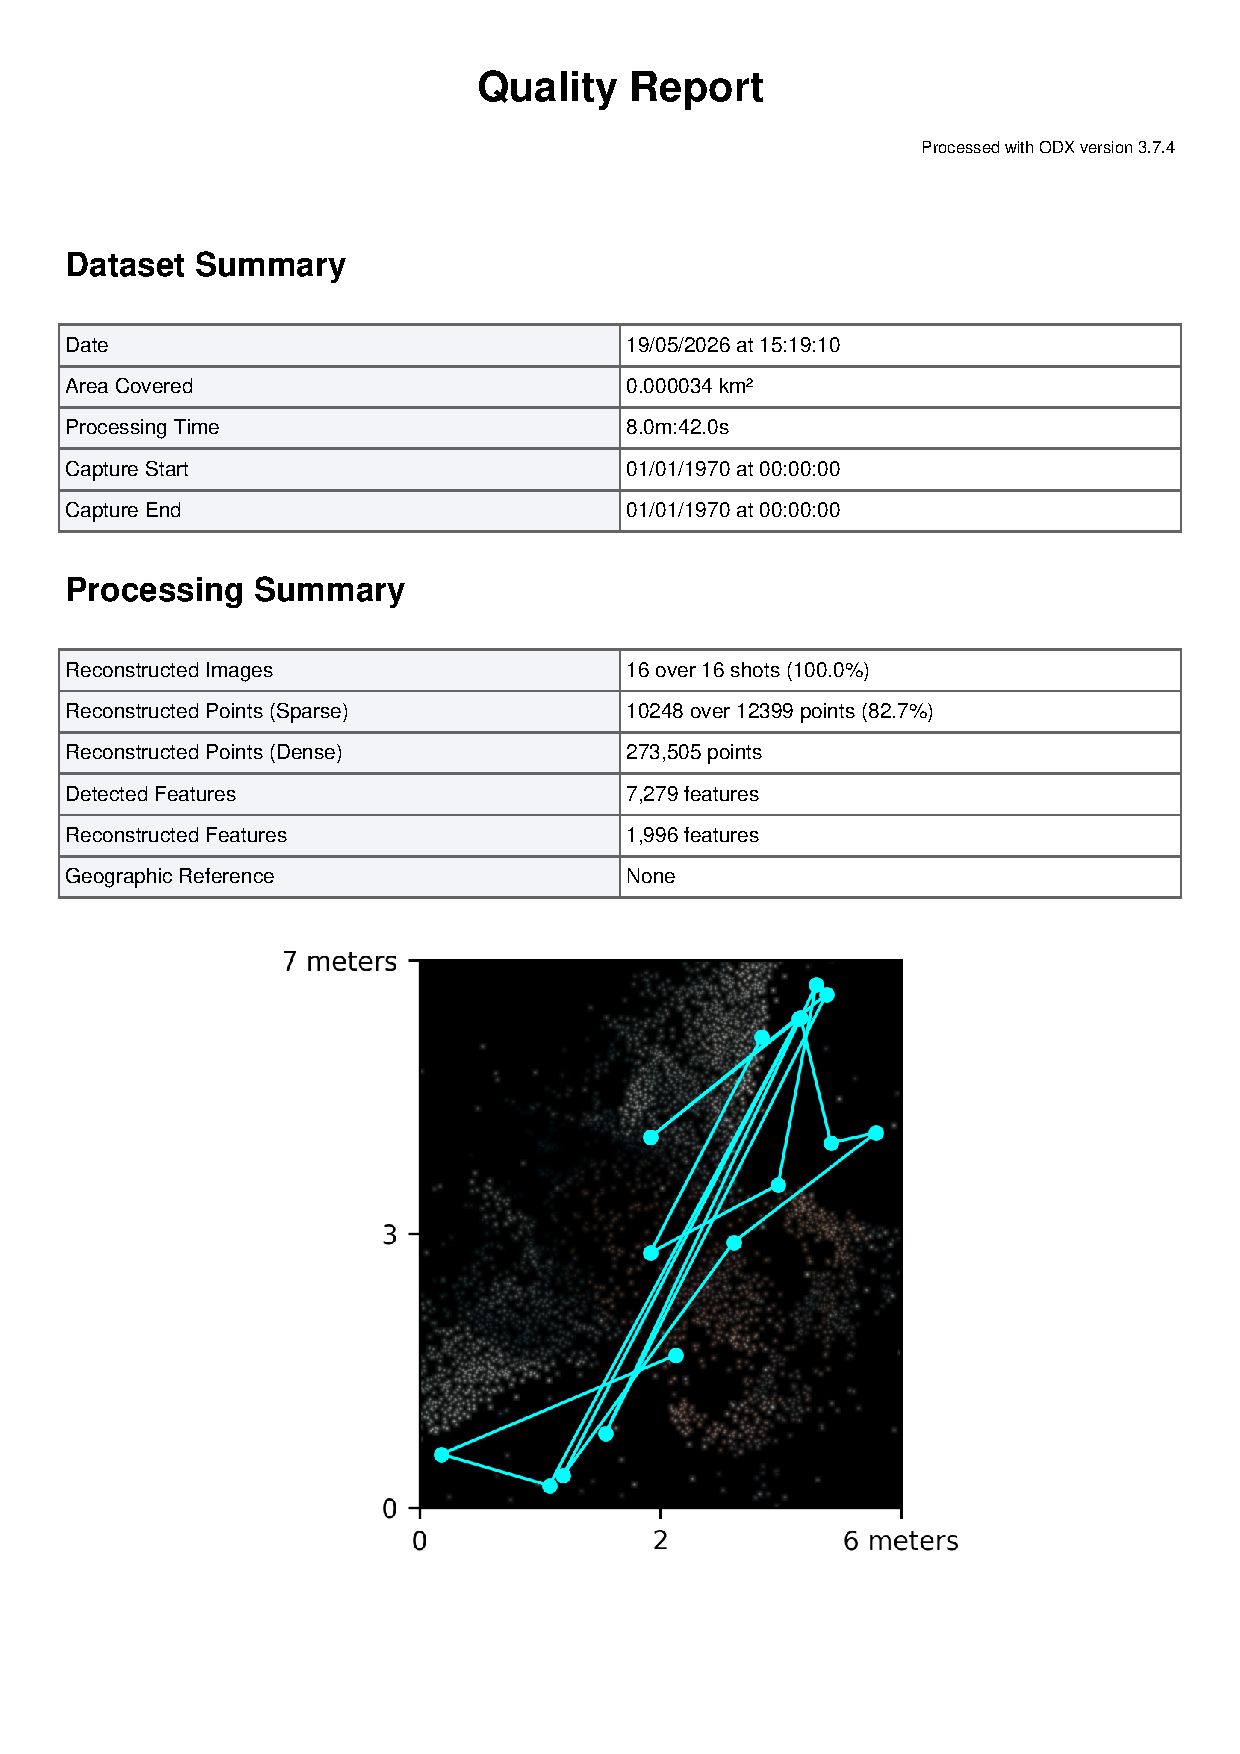
\includepdf[pages=-,fitpaper=true,pagecommand={\thispagestyle{fancy}}]{webodm_quality_report.pdf}

\end{document}
